\documentclass[DaoFP]{subfiles}
\begin{document}
 \setcounter{chapter}{18}

 \chapter{Kan Extensions(Kan扩展)}

 如果说范畴论不断提高抽象层次,是因为它的核心在于发现模式。一旦发现了模式,接下来就是研究这些模式所形成的更高层次的模式,依此类推。

 我们已经看到相同的概念在更高的抽象层次上以越来越简洁的方式重复出现。

 例如,我们最初使用泛范构造(universal construction)定义了积(product)。然后我们看到在积的定义中涉及的跨度(span)实际上是自然变换(natural transformations)。这引导我们将积解释为极限(limit)。接着我们又看到,可以用伴随(adjunctions)来定义它。我们最终能够用一个简洁的公式将积与余积(coproduct)结合起来:
 \[ (+) \dashv \Delta \dashv (\times) \]
 老子说过:“将欲取之,必先与之。”

 Kan扩展进一步提高了抽象的层次。Mac Lane 曾说:“所有的概念都是 Kan 扩展。”

 \section{Closed Monoidal Categories(闭单态范畴)}

 我们已经看到,如何将一个函数对象定义为范畴积(categorical product)的右伴随(right adjoint):
 \[ \cat C (a \times b, c) \cong \cat C (a, [b, c]) \]
 这里我使用了一个替代符号 $[b, c]$ 来表示内部同态(internal hom),即指数(exponential)$c^b$。

 两个函子的伴随关系可以被认为是其中一个函子的伪逆(pseudo-inverse)。它们的组合并不形成恒等映射,但它们的组合通过单位(unit)和余单位(counit)与恒等函子相关联。例如,如果你仔细观察,柯里化(currying)伴随的余单位:
 \[ \varepsilon_{b c} \colon [b, c] \times b \to c \]
 表明$[b, c]$在某种意义上体现了乘法的逆。它的作用类似于除法中的$c/b$:
 \[ c/b \times b = c \]

 以典型的范畴论方式,我们可能会问:如果我们将积替换为其他东西会怎样?显而易见,将它替换为余积(coproduct)是行不通的(因此我们没有减法的类比)。但也许还有其他行为良好的二元运算可以有一个右伴随。

 一种自然的推广积的方式是使用具有张量积(tensor product)$\otimes$ 和单位对象 $I$ 的单态范畴(monoidal category)。如果存在一个伴随关系:
 \[ \cat C (a \otimes b, c) \cong \cat C (a, [b, c]) \]
 我们将该范畴称为闭单态(closed monoidal)范畴。除非引起混淆,典型的范畴论中滥用符号,我们将继续使用相同的符号(方括号)来表示单态内部同态(monoidal internal hom),就像我们在笛卡尔积(cartesian hom)中所做的那样。还有一种替代的符号表示法,称为棒棒糖(lollipop)符号,用来表示张量积的右伴随:
 \[ \cat C (a \otimes b, c) \cong \cat C (a, b \multimap c) \]
 它通常在\emph{线性类型}(linear types)的上下文中使用。

 内部同态的定义适用于对称单态范畴(symmetric monoidal category)。如果张量积不是对称的,伴随关系定义了\emph{左闭单态}范畴。左内部同态(left internal hom)是“后乘法”函子$(- \otimes b)$的右伴随。右闭结构则定义为“前乘法”函子$(b \otimes -)$的右伴随。如果两者都定义了,那么该范畴称为\emph{双闭单态范畴}(bi-closed monoidal category)。

 \subsection{Internal Hom for Day Convolution(Day 卷积的内部同态)}

 作为一个例子,考虑具有Day卷积(Day convolution)的协预层(co-presheaves)范畴中的对称单态结构:
 \[ (F \star G) x = \int^{a, b} \cat C (a \otimes b, x) \times F a \times G b \]
 我们正在寻找伴随关系:
 \[ [\cat C, \Set] (F \star G, H) \cong  [\cat C, \Set] (F, [G, H]_{\text{Day}}) \]
 左边的自然变换可以写成$x$上的一个末端(end):
 \[ \int_x \Set \big( \int^{a, b} \cat C (a \otimes b, x) \times F a \times G b, H x \big) \]
 我们可以利用共连续性(co-continuity)将共末端(coend)提取出来:
 \[ \int_{x, a, b} \Set \big( \cat C (a \otimes b, x) \times F a \times G b, H x \big) \]
 接下来我们使用$\Set$中的柯里化伴随(currying adjunction):
 \[ \int_{x, a, b} \Set \big( F a, [\cat C (a \otimes b, x)  \times G b, H x] \big) \]
 最后,我们使用同态集的连续性(continuity of the hom-set)将两个末端移到同态集(hom-set)的内部:
 \[ \int_{a} \Set \big( F a, \int_{x, b} [\cat C (a \otimes b, x)  \times G b, H x] \big) \]
 我们发现Day卷积的右伴随由以下给出:
 \[ \big([G, H]_{\text{Day}}\big) a = \int_{x, b} \big[\cat C(a \otimes b, x), [G b, H x]\big] \cong \int_b [G b, H (a \otimes b)] \]
 最后的转换是应用$\Set$中的Yoneda引理(Yoneda lemma)。

 \begin{exercise}
  实现Day卷积的内部同态在Haskell中的实现。提示:使用类型别名。
 \end{exercise}

 \begin{exercise}
  实现以下伴随关系的见证:
  \begin{haskell}
   ltor :: (forall a. Day f g a -> h a) -> (forall a. f a -> DayHom g h a)
   rtol :: Functor h =>
   (forall a. f a -> DayHom g h a) -> (forall a. Day f g a -> h a)
  \end{haskell}
 \end{exercise}

 \subsection{Powering and Co-powering(冪对象与余冪对象)}

 在集合范畴(Set)中,内部同态(function object)等价于外部同态(external hom),即两个对象之间的态射集:
 \[ C^B \cong Set(B, C) \]
 因此我们可以将定义集合范畴中内部同态的柯里化伴随关系改写为:
 \[ \Set (A \times B, C)  \cong \Set \big(A, \Set (B, C)\big) \]
 我们可以将此伴随关系推广到$B$和$C$不再是集合,而是一些范畴$\cat C$中的对象的情况。任何范畴中的外部同态总是一个集合。然而,左边不再由积定义。相反,它定义了一个集合$A$作用于对象$b$上的行为:
 \[ \cat C (A \cdot b, c) \cong \Set \big( A, \cat C (b, c)\big) \]
 这被称为\emph{余冪}(co-power)。

 你可以将这种行为理解为将$A$个$b$相加在一起(取它们的余积)。例如,如果$A$是一个包含两个元素的集合$\mathbf 2$,我们得到:
 \[ \cat C (\mathbf 2 \cdot b, c) \cong \Set \big( \mathbf 2, \cat C (b, c)\big) \cong \cat C(b, c) \times \cat C(b, c) \cong \cat C(b + b, c) \]
 换句话说,
 \[ \mathbf 2 \cdot b \cong b + b \]
 从这个意义上说,余冪定义了迭代加法形式的乘法,就像我们在学校里学到的一样。

 如果我们将$b$乘以同态集$\cat C (b, c)$并对所有$b$取共末端,结果同构于$c$:
 \[ \cat \int^b C(b, c) \cdot b \cong c \]
 实际上,由于Yoneda引理,两边到任意$x$的映射是同构的:
 \[ \cat C \big( \int^b \cat C(b, c) \cdot b, x\big) \cong \int_b \Set \big( \cat C(b, c), \cat C (b, x)\big) \cong \cat C (c, x)\]

 正如预期的那样,在集合范畴中,余冪简化为笛卡尔积(cartesian product)。
 \[ \Set (A \cdot B, C) \cong \Set \big( A, \Set(B, C)\big) \cong \Set (A \times B, C) \]

 类似地,我们可以将冪对象(power)表达为迭代乘法。我们使用相同的右侧,但这次我们用映射来定义\emph{冪}:
 \[ \cat C (b, A \pitchfork c) \cong \Set  \big(A, \cat C(b, c)\big) \]
 你可以将冪理解为将$A$个$c$相乘在一起。实际上,将$A$替换为$\mathbf 2$的结果是:
 \[ \cat C (b, \mathbf 2 \pitchfork c) \cong \Set  \big(\mathbf 2, \cat C(b, c)\big) \cong \cat C(b, c) \times \cat C(b, c) \cong \cat C (b, c \times c)\]
 换句话说:
 \[ \mathbf 2 \pitchfork c \cong c \times c \]
 这是一种表示$c^2$的花式写法。

 如果我们将$c$乘以同态集$\cat C(c', c)$并对所有$c$取末端,结果同构于$c'$:
 \[ \int_c \cat C (c', c) \pitchfork c \cong c' \]
 这可以从Yoneda引理中得出。实际上,从$x$到两边的映射是同构的:
 \[ \cat C \big(x, \int_c \cat C (c', c) \pitchfork c\big) \cong \int_c \Set \big( \cat C(c', c), \cat C(x, c)\big)  \cong \cat C (x, c') \]

 在集合范畴中,冪简化为指数(exponential),它与同态集是同构的:
 \[ A \pitchfork C \cong C^A \cong \Set (A, C) \]
 这是因为乘法的对称性所致。
 \[ \Set(B, A \pitchfork C) \cong \Set (A, \Set(B, C)) \cong \Set (A \times B, C) \]
 \[ \cong \Set (B \times A, C) \cong \Set (B, \Set (A, C))\]

 \section{Inverting a Functor(反转一个函子)}

 范畴论的一个方面是通过执行有损转换丢弃信息;另一个方面是恢复丢失的信息。我们已经看到用自由函子(free functors)补偿丢失数据的例子——这是遗忘函子(forgetful functors)的伴随函子。Kan扩展是另一个例子。两者都弥补了那些不可逆函子丢失的数据。

 一个函子可能不可逆的原因有两个。一个是它可能将多个对象或箭头映射到单个对象或箭头上。换句话说,它在对象或箭头上不是单射的(injective)。另一个原因是它的像可能无法覆盖整个目标范畴。换句话说,它在对象或箭头上不是满射的(surjective)。

 例如,考虑一个伴随$L \dashv R$。假设$R$不是单射的,它将两个对象$c$和$c'$合并为一个对象$d$
 \begin{align*}
  R c &= d \\
  R c' &= d
 \end{align*}
 $L$无力逆转这种操作。它无法同时将$d$映射到$c$和$c'$。它最多只能将$d$映射到一个“更一般”的对象$L d$,该对象有箭头指向$c$和$c'$。这些箭头用于定义伴随的余单位的分量:
 \begin{align*}
  \varepsilon_c &\colon L d \to c
  \\
  \varepsilon_{c'} &\colon L d \to c'
 \end{align*}
 其中$L d$既是$L (R c)$也是$L (R c')$
 \[
  \begin{tikzcd} [row sep=0.5cm, column sep=1cm]
   L d
   \arrow[d, "\varepsilon_c"]
   \arrow[dd, bend right, "\varepsilon_{c'}"']
   \\
   c
   \arrow[rr, red, dashed, ""]
   && d
   \arrow[ull, blue, bend right, dashed, "L"']
   \\
   c'
   \arrow[urr, red, bend right, dashed, "R"]
  \end{tikzcd}
 \]

 此外,如果$R$在对象上不是满射的,函子$L$必须以某种方式在$R$的像之外的$\cat D$对象上进行定义。同样,单位和余单位的自然性会限制可能的选择,只要这些对象与$R$的像有箭头连接。

 显然,所有这些限制意味着伴随只能在非常特殊的情况下定义。

 Kan扩展甚至比伴随还要弱。

 如果伴随函子像逆一样工作,Kan扩展就像分数一样工作。

 这在我们重绘定义伴随的余单位和单位的图表时看得最清楚。在第一个图中,$L$似乎扮演了$1/R$的角色。在第二个图中,$R$则假装自己是$1/L$。

 \[
  \begin{tikzcd} [row sep=1cm, column sep=1cm]
   \cat C
   \arrow[rr, "\text{Id}", "" {name=ID, below} ]
   \arrow[d, bend right, "R"']
   && \cat C
   \\
   \cat D
   \arrow[urr, bend right, "L"']
   \arrow[Rightarrow, "\varepsilon",  to=ID]
  \end{tikzcd}
  \qquad
  \begin{tikzcd} [row sep=1cm, column sep=1cm]
   \cat D
   \arrow[rr, "\text{Id}", "" {name=ID, below} ]
   \arrow[d, bend right, "L"']
   && \cat D
   \\
   \cat C
   \arrow[urr, bend right, "R"']
   \arrow[Rightarrow, "\eta",  from=ID]
  \end{tikzcd}
 \]

 右Kan扩展$\text{Ran}_P F$和左Kan扩展$\text{Lan}_P F$通过将恒等函子替换为某个函子$F \colon \cat E \to \cat C$来推广这些概念。Kan扩展扮演的角色类似于分数$F/P$。从概念上讲,它们“逆转”$P$的作用,并跟随它执行$F$的作用。

 \[
  \begin{tikzcd} [row sep=1cm, column sep=1cm]
   \cat E
   \arrow[rr, "F", "" {name=ID, below} ]
   \arrow[d, bend right, "P"']
   && \cat C
   \\
   \cat B
   \arrow[urr, bend right, "\text{Ran}_P F"']
   \arrow[Rightarrow, "\varepsilon",  to=ID]
  \end{tikzcd}
  \qquad
  \begin{tikzcd} [row sep=1cm, column sep=1cm]
   \cat E
   \arrow[rr, "F", "" {name=ID, below} ]
   \arrow[d, bend right, "P"']
   && \cat C
   \\
   \cat B
   \arrow[urr, bend right, "\text{Lan}_P F"']
   \arrow[Rightarrow, "\eta",  from=ID]
  \end{tikzcd}
 \]

 正如伴随的情况一样,“逆转”并不完全。组合$\text{Ran}_P F \circ P$并不能还原$F$;相反,它通过一个称为余单位(counit)的自然变换$\varepsilon$与它相关联。同样,组合$\text{Lan}_P F \circ P$通过单位(unit)$\eta$与$F$相关联。

 请注意,$F$丢弃的信息越多,Kan扩展“逆转”函子$P$就越容易。在某种意义上,它只需“模$F$”逆转$P$即可。

 以下是关于Kan扩展的直觉。我们从一个函子$F$开始:
 \[
  \begin{tikzcd} \cat E
  \arrow[r, "F"]
  & \cat C
  \end{tikzcd}
 \]
 有一个第二个函子$P$,它将$\cat E$压缩到另一个范畴$\cat B$中。这可能是一个嵌入,它是有损且非满射的。我们的任务是以某种方式\emph{扩展} $F$的定义,以涵盖整个$\cat B$。

 在理想情况下,我们希望以下图表能够交换:
 \[
  \begin{tikzcd} \cat E
  \arrow[r, "F"]
  \arrow[d, "P"']
  & \cat C
  \\
  \cat B
  \arrow[ur, "Kan_P F"']
  \end{tikzcd}
 \]
 但这会涉及函子之间的相等,这是我们尽量避免的。

 下一个最好的选择是要求在这个图中两条路径之间存在一个自然同构。但是即使这样看起来也要求过高。因此,我们最终决定要求一条路径能够变形为另一条路径,这意味着它们之间存在一个单向的自然变换。这种变换的方向区分了右Kan扩展和左Kan扩展。

 \section{Right Kan Extension(右Kan扩展)}

 右Kan扩展是一个函子$\text{Ran}_P F$,配备了一个自然变换$\varepsilon$,称为Kan扩展的余单位,定义为:
 \[ \varepsilon \colon (\text{Ran}_P F) \circ P \to F\]
 \[
  \begin{tikzcd} [row sep=1cm, column sep=1cm]
   \cat E
   \arrow[rr, "F", "" {name=ID, below} ]
   \arrow[d, bend right, "P"']
   && \cat C
   \\
   \cat B
   \arrow[urr, blue, bend right, "\text{Ran}_P F"']
   \arrow[Rightarrow, blue, "\varepsilon",  to=ID]
  \end{tikzcd}
 \]

 对$\text{Ran}_P F$的要求是,$(\text{Ran}_P F, \varepsilon)$在所有类似对$(G, \alpha)$中是泛化的,其中$G$是一个函子$G \colon \cat B \to \cat C$,而$\alpha$是一个自然变换:
 \[ \alpha \colon G \circ P \to F \]
 \[
  \begin{tikzcd} [row sep=1cm, column sep=1cm]
   \cat E
   \arrow[rr, "F", "" {name=ID, below} ]
   \arrow[d, bend right, "P"']
   && \cat C
   \\
   \cat B
   \arrow[urr, red, bend right, "G"']
   \arrow[Rightarrow, red, "\alpha",  to=ID]
  \end{tikzcd}
 \]

 泛化意味着对于任何这样的$(G, \alpha)$,都存在唯一的自然变换$\sigma \colon G \to \text{Ran}_P F$,
 \[
  \begin{tikzcd}[row sep=2cm, column sep=2cm]
   \cat E  \ar[d, bend right, "P"', "" {name=P}]
   \ar[r, "F", ""  {name=F, below, near start, bend right}]
   &
   \cat C
   \\
   \cat B
   \ar[ur, red, bend left, "G", "" {name=G, below}]
   \ar[ur, blue, bend right, "\text{Ran}_P F"', "" {name=Ran}]
   \arrow[Rightarrow, "\sigma", from=G, to=Ran]
  \end{tikzcd}
 \]
 它使得$\alpha$可以分解为:
 \[ \alpha = \varepsilon \cdot (\sigma \circ P) \]
 这是一个在自然变换的垂直和水平组合中,其中$\sigma \circ P$是$\sigma$的卷须(whiskering)。以下是相同的方程式,用线图的方式绘制:

 \[
  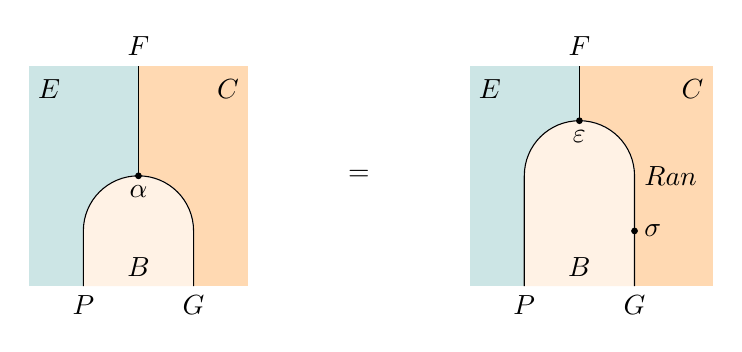
\begin{tikzpicture}
   \def \dx {0.7}
   \def \dy {0.7}

   \def \xa{-3 * \dx};
   \def \xb{-2 * \dx};
   \def \xc{-1 * \dx};
   \def \xd{0};
   \def \xe{1 * \dx};

   \def \ya{0};
   \def \yb{1 * \dy};
   \def \yc{2 * \dy};
   \def \yd{3 * \dy};
   \def \ye{4 * \dy};

% left background
   \filldraw[fill=blue!50!green!20, draw=white] (\xa, \ye) rectangle (\xc, \ya);
% right background
   \filldraw[fill=orange!30, draw=white] (\xc, \ye) rectangle (\xe, \ya);
% fill shape\yb
   \path [fill=orange!10, draw=white]  (\xb, \ya) to (\xb, \yb) to [out=90, in=180]  (\xc, \yc) to  [out=0, in=90] (\xd, \yb) to (\xd, \ya);

% cup
   \draw (\xb, \ya) to (\xb, \yb) to [out=90, in=180]  (\xc, \yc) to  [out=0, in=90] (\xd, \yb) to (\xd, \ya);
   \draw (\xc, \yc) -- (\xc, \ye);

% natural transformations
   \filldraw[black] (\xc, \yc) circle (1 pt);
   \node [below] at (\xc, \yc) {$\alpha$};

% categories
   \node[right] at (\xa, \ye - 0.3) {$\cat E$};
   \node[left] at (\xe, \ye - 0.3) {$\cat C$};
   \node[above] at (\xc, \ya) {$\cat B$};
% functors
   \node [below] at (\xb, \ya) {$P$};
   \node [below] at (\xd, \ya) {$G$};
   \node [above] at (\xc, \ye) {$F$};

%-----------------
   \node (eq) at (3 * \dx, \yc) {$=$};
% right diagram

   \def \xa{5 * \dx};
   \def \xb{6 * \dx};
   \def \xc{7 * \dx};
   \def \xd{8 * \dx};
   \def \xe{9 * \dx + 0.3};

% left background
   \filldraw[fill=blue!50!green!20, draw=white] (\xa, \ye) rectangle (\xc, \ya);
% right background
   \filldraw[fill=orange!30, draw=white] (\xc, \ye) rectangle (\xe, \ya);
% fill shape
   \path [fill=orange!10, draw=white]  (\xb, \ya) to (\xb, \yc) to [out=90, in=180]  (\xc, \yd) to  [out=0, in=90] (\xd, \yc) to (\xd, \ya);

% cup
   \draw (\xb, \ya) to (\xb, \yc) to [out=90, in=180]  (\xc, \yd) to  [out=0, in=90] (\xd, \yc) to (\xd, \ya);
   \draw (\xc, \yd) -- (\xc, \ye);

% natural transformations
   \filldraw[black] (\xc, \yd) circle (1 pt);
   \node [below] at (\xc, \yd) {$\varepsilon$};

   \filldraw[black] (\xd, \yb) circle (1 pt);
   \node [right] at (\xd, \yb) {$\sigma$};

% categories
   \node[right] at (\xa, \ye - 0.3) {$\cat E$};
   \node[left] at (\xe, \ye - 0.3) {$\cat C$};
   \node[above] at (\xc, \ya) {$\cat B$};
% functors
   \node [below] at (\xb, \ya) {$P$};
   \node [below] at (\xd, \ya) {$G$};
   \node [above] at (\xc, \ye) {$F$};
   \node [right] at (\xd, \yc) {$\text{Ran}$};

  \end{tikzpicture}
 \]

 如果沿$P$的右Kan扩展对每个函子$F$都定义了,那么这个泛范构造可以推广到一个伴随关系——这次它是在两个函子范畴之间的伴随关系:
 \[ [\cat E, \cat C](G \circ P, F) \cong [\cat B, \cat C](G, \text{Ran}_P F) \]
 对于任何$\alpha$(左侧的元素),都存在唯一的$\sigma$(右侧的元素)。

 换句话说,如果右Kan扩展对每个$F$都存在,那么它就是函子前组合的右伴随:
 \[ (- \circ P) \dashv \text{Ran}_P \]
 这个伴随关系的余单位在$F$的成分就是$\varepsilon$。

 这在某种程度上类似于柯里化伴随:
 \[ \cat E (a \times b, c) \cong \cat E (a, [b, c]) \]
 其中积被函子组合取代。(这个类比并不完美,因为组合只能在自函子范畴中被认为是张量积。)

 \subsection{Right Kan Extension as an End(作为末端的右Kan扩展)}

 回顾一下忍者Yoneda引理:
 \[ F b \cong \int_{e} \mathbf{Set} (\cat B(b, e), F e) \]
 这里,$F$是一个协预层,即从$\cat B$到$\Set$的函子。沿$P$的$F$的右Kan扩展推广了这个公式:
 \[ (\text{Ran}_P F) b \cong \int_e \Set \big( \cat B (b, P e), F e\big) \]

 这适用于协预层。通常我们关心的是$F \colon \cat E \to \cat C$,因此我们需要将$\Set$中的同态集替换为\emph{冪}(power)。因此,右Kan扩展由以下末端给出(如果它存在的话):
 \[ (\text{Ran}_P F) b \cong \int_e \cat B (b, P e) \pitchfork F e \]

 证明基本上是自然而然的:在每一步中只有一种操作可以执行。我们从伴随开始:
 \[ [\cat E, \cat C](G \circ P, F) \cong [\cat B, \cat C](G, \text{Ran}_P F) \]
 并使用末端重新书写它:
 \[ \int_e \cat C \big(G ( P e), F e\big) \cong \int_b \cat C\big(G b, (\text{Ran}_P F) b\big) \]
 我们将我们的公式代入得到:
 \[ \cong  \int_b \cat C\big(G b,\int_e \cat B (b, P e) \pitchfork F e \big)\]
 我们使用同态函子的连续性将末端推到前面:
 \[  \cong  \int_b \int_e \cat C\big(G b, \cat B (b, P e) \pitchfork F e \big) \]
 然后我们使用冪的定义:
 \[ \int_b \int_e \Set \big(  \cat B (b, P e), \cat C (G b, F e) \big) \]
 并应用Yoneda引理:
 \[ \int_e  \cat C \big(G (P e), F e\big) \]
 这个结果确实是伴随关系的左侧。

 如果$F$是一个协预层,右Kan扩展公式中的冪简化为指数/同态集:
 \[ (\text{Ran}_P F) b \cong \int_e \Set \big( \cat B (b, P e), F e\big) \]

 还要注意的是,如果$P$有一个左伴随,我们称之为$P^{-1}$,即:
 \[ \cat B(b, P e) \cong \cat E(P^{-1} b, e) \]
 我们可以使用忍者Yoneda引理来计算末端:
 \[ (\text{Ran}_P F) b \cong \int_e \Set \big( \cat B (b, P e), F e\big) \cong \int_e \Set(\cat E(P^{-1} b, e), F e) \cong F(P^{-1} b)\]
 得到:
 \[  \text{Ran}_P F \cong F \circ P^{-1} \]
 由于伴随关系是逆的弱化,这个结果与Kan扩展“逆转”$P$并跟随$F$的直觉是一致的。

 \subsection{Right Kan extension in Haskell(Haskell中的右Kan扩展)}

 右Kan扩展的末端公式可以直接翻译为Haskell代码:
 \begin{haskell}
  newtype Ran p f b = Ran (forall e. (b -> p e) -> f e)
 \end{haskell}

 右Kan扩展的余单位$\varepsilon$是一个从\hask{(Ran p f)}和\hask{p}的组合到\hask{f}的自然变换:
 \begin{haskell}
  counit :: forall p f e'. Ran p f (p e') -> f e'
 \end{haskell}
 为了实现它,我们需要生成一个类型为\hask{(f c')}的值,给定一个多态函数
 \begin{haskell}
  h :: forall e. (p e' -> p e) -> f e
 \end{haskell}
 我们通过在类型\hask{e = e'}上实例化此函数并用\hask{(p e')}上的身份函数调用它来实现:
 \begin{haskell}
  counit (Ran h) = h id
 \end{haskell}

 右Kan扩展的计算能力来自其泛性质。我们从一个带有自然变换的函子$G$开始:
 \[ \alpha \colon G \circ P \to F \]
 这可以表示为一个Haskell数据类型:
 \begin{haskell}
  type Alpha p f g = forall e. g (p e) -> f e
 \end{haskell}
 泛化性质告诉我们,存在一个唯一的自然变换$\sigma$,从这个函子到相应的右Kan扩展:
 \begin{haskell}
  sigma :: Functor g => Alpha p f g -> forall b. (g b -> Ran p f b)
  sigma alpha gb = Ran (\b_pe -> alpha $ fmap b_pe gb)
 \end{haskell}
 该变换通过余单位$\varepsilon$分解$\alpha$:
\[ \alpha = \varepsilon \cdot (\sigma \circ P) \]
请记住,卷须(whiskering)意味着我们在\hask{b = p c}时实例化\hask{sigma}。然后它跟随\hask{counit}。$\alpha$的分解由下式给出:
\begin{haskell}
factorize' :: Functor g => Alpha p f g -> forall e. g (p e) -> f e
factorize' alpha gpc = alpha gpc
\end{haskell}

这三个自然变换的成分都是目标范畴$\cat C$中的态射:
\[
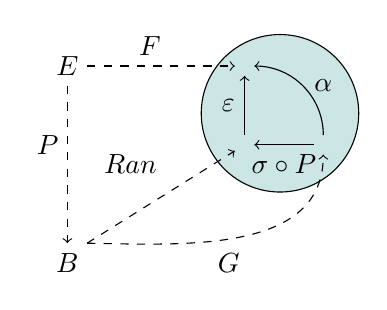
\begin{tikzpicture}
\def\Xa{0};
\def\Xm{1.3}
\def\Xb{2.25};
\def\Xc{3};
\def\Yc{2.5};
\def\Yb{1.75};
\def\Ya{0};

\node at ( \Xa, \Yc) { $\cat E$ };
\node at ( \Xa, \Ya) { $\cat B$ };
\node (1) at (\Xb, \Yc) {};
\node (2) at (\Xb, \Yb - 0.25) {};
\node (3) at (\Xb + 1, \Yb - 0.25) {};

\draw (\Xc - 0.3, \Yc - 0.6)[fill=blue!50!green!20]  ellipse (1 and 1);

% F
\node at ( \Xm-0.25, \Yc + 0.25) { $F$ };
\draw[->, dashed](\Xa + 0.25, \Yc) -- (1);
% P
\node at (\Xa - 0.25, \Yb - 0.25) { $P$ };
\draw[->, dashed](\Xa, \Yc - 0.25) -- (\Xa, \Ya + 0.25);
% Ran
\node at (\Xm - 0.5, \Yb - 0.5) { $\text{Ran}$ };
\draw[->, dashed](\Xa + 0.25, \Ya + 0.25) -- (2);

% G
\node at (\Xb - 0.2, \Ya) { $\text{G}$ };
\draw[->, dashed](\Xa + 0.25, \Ya + 0.25) to [out=-1, in=-90] (3);

\draw[->] (2) -- (1) node[midway, left] {$\varepsilon$};
\draw[->] (3) -- (2) node[midway, below] {$\sigma \circ P$};
\draw[->] (3) to [out=90, in=0] (1);
\node at (\Xb + 1, \Yb + 0.5) {$\alpha$};
\end{tikzpicture}
\]

\begin{exercise}
Implement the \hask{Functor} instance for \hask{Ran}.
\end{exercise}

\subsection{Limits as Kan extensions(作为Kan扩展的极限)}
我们之前已经定义了极限(limits)为泛锥(universal cones)。锥的定义涉及两个范畴:定义图形的指标范畴$\cat J$和目标范畴$\cat C$。图(diagram)是一个函子$D \colon \cat J \to \cat C$,它将形状嵌入目标范畴中。

我们可以引入第三个范畴$\mathbf 1$:一个包含单个对象和单个恒等箭头的终范畴。然后我们可以使用从该范畴到锥顶点$x$的函子$X$。由于$\mathbf 1$在$\mathbf{Cat}$中是终范畴,因此我们也有从$\cat J$到它的唯一函子,我们称之为$!$。它将所有对象映射到$\mathbf 1$的唯一对象,并将所有箭头映射到其恒等箭头。

事实证明,$D$的极限是沿着$!$的图$D$的右Kan扩展。首先,观察组合$X \circ !$将形状$\cat J$映射到单个对象$x$,因此它充当了常函子$\Delta_x$的作用。它选择锥的顶点。一个以$x$为顶点的锥是一个自然变换$\gamma$:
\[
\begin{tikzcd} [row sep=1cm, column sep=1cm]
\cat J
\arrow[rr, "D", "" {name=ID, below} ]
\arrow[d, bend right, "!"']
&& \cat C
\\
\mathbf 1
\arrow[urr, bend right, "X"']
\arrow[Rightarrow, "\gamma",  to=ID]
\end{tikzcd}
\]

下图说明了这一点。左图中有两个范畴:具有单个对象$*$的$\mathbf 1$和具有三个对象形成图形的$\cat J$。右图中有$D$的图像和$X \circ !$的图像,即顶点$x$。$\gamma$的三个成分将顶点$x$连接到图上。$\gamma$的自然性确保形成锥边的三角形是交换的。

\[
\begin{tikzcd}
& *
\\
\\
1
\arrow[rr, red]
\arrow[rd, red]
&& 2
\arrow[dl, red]
\\
& 3
\end{tikzcd}
\qquad
\begin{tikzcd}
& x
\arrow[ddr, "\gamma_2"]
\arrow[ddl, "\gamma_1"']
\arrow[ddd, "\gamma_3"]
\\
\\
D 1
\arrow[rr, red]
\arrow[rd, red]
&& D 2
\arrow[dl, red]
\\
& D 3
\end{tikzcd}
\]

右Kan扩展$(\text{Ran}_! D, \varepsilon)$是泛化的这种锥。$\text{Ran}_! D$是一个从$\mathbf 1$到$\cat C$的函子,因此它选择$\cat C$中的一个对象。这确实是泛锥的顶点$\text{Lim} D$。

泛化性意味着对于任何对$(X, \gamma)$,都有一个自然变换$\sigma \colon X \to \text{Ran}_! D$
\[
\begin{tikzcd}[row sep=2cm, column sep=2cm]
\cat J  \ar[d, "!"', "" {name=P}]
\ar[r, "D", ""  {name=F, below, near start, bend right}]
&
\cat C
\\
\mathbf 1
\ar[ur, bend left, "X", "" {name=G, below}]
\ar[ur, bend right, "\text{Ran}_! D"', "" {name=Ran}]
\arrow[Rightarrow, "\sigma", from=G, to=Ran]
\end{tikzcd}
\]
它分解$\gamma$。

变换$\sigma$只有一个成分$\sigma_*$,它是将顶点$x$连接到顶点$\text{Lim} D$的箭头$h$。分解如下:
\[ \gamma = \varepsilon \cdot (\sigma \circ !) \]
以分量的形式:
\[ \gamma_i = \varepsilon_i \circ h \]
它使下图中的三角形交换:
\[
\begin{tikzcd}[row sep=1cm]
& x
\arrow[dddl, "\gamma_1"']
\arrow[ddddr, "\gamma_3"]
\arrow[dddrr, "\gamma_2"]
\arrow[dd, dashed, "h"']
\\
\\
& \text{Lim} D
\arrow[dl, blue, "\varepsilon_1"]
\arrow[ddr, blue, "\varepsilon_3"']
\arrow[drr, blue, "\varepsilon_2"]
\\
D 1
\arrow[rrr, red]
\arrow[rrd, red]
&&& D 2
\arrow[dl, red]
\\
&& D 3
\end{tikzcd}
\]
这种泛化条件使$\text{Lim} D$成为图$D$的极限。

\subsection{Left adjoint as a right Kan extension(作为右Kan扩展的左伴随)}

我们开始描述Kan扩展作为伴随的推广。观察这些图,如果我们有一对伴随函子$L \dashv R$,我们希望左函子是沿右函子的恒等函子的右Kan扩展。
\[ L \cong \text{Ran}_R \text{Id} \]
实际上,Kan扩展的余单位与伴随的余单位相同:

\[
\begin{tikzcd} [row sep=1cm, column sep=1cm]
\cat C
\arrow[rr, "\text{Id}", "" {name=ID, below} ]
\arrow[d, bend right, "R"']
&& \cat C
\\
\cat D
\arrow[urr, bend right, "L"']
\arrow[Rightarrow, "\varepsilon",  to=ID]
\end{tikzcd}
\]
我们还需要展示泛化性:
\[
\begin{tikzcd} [row sep=1cm, column sep=1cm]
\cat C
\arrow[rr, "\text{\text{Id}}", "" {name=ID, below} ]
\arrow[d, bend right, "R"']
&& \cat C
\\
\cat D
\arrow[urr, bend right, "G"']
\arrow[Rightarrow, "\alpha",  to=ID]
\end{tikzcd}
\qquad %----%
\begin{tikzcd}[row sep=2cm, column sep=2cm]
\cat C  \ar[d, "R"', "" {name=P}]
\ar[r, "R", ""  {name=F, below, near start, bend right}]
&
\cat D
\\
\cat D
\ar[ur, bend left, "G", "" {name=G, below}]
\ar[ur, bend right, "L"', "" {name=Ran}]
\arrow[Rightarrow, "\sigma", from=G, to=Ran]
\end{tikzcd}
\]
为此,我们可以使用伴随的单位:
\[ \eta \colon \text{Id} \to R \circ L \]
我们将$\sigma$构造为复合:
\[ G \rightarrow G \circ \text{Id} \xrightarrow{G \circ \eta} G \circ R \circ L \xrightarrow{\alpha \circ L} \text{Id} \circ L \rightarrow L\]
换句话说,我们将$\sigma$定义为:
\[ \sigma = (\alpha \circ L) \cdot (G \circ \eta) \]

我们可以问反向问题:如果$\text{Ran}_R \text{Id}$存在,它是否自动成为$R$的左伴随?事实证明,为此我们需要一个额外的条件:Kan扩展必须被$R$保留,即:
\[ R \circ \text{Ran}_R \text{Id} \cong \text{Ran}_R R \]
我们将在下一节中看到这个条件的右侧定义了密度余子模。

\begin{exercise}
Show the factorization condition:
\[ \alpha = \varepsilon \cdot (\sigma \circ R) \]
for the $\sigma$ that was defined above. Hint: draw the corresponding string diagrams and use the triangle identity for the adjunction.
\end{exercise}

\subsection{Codensity monad(密度余子模)}

我们已经看到,每个伴随$L \dashv F$都会产生一个子模$F \circ L$。事实证明,这个子模是沿$F$的$F$的右Kan扩展。有趣的是,即使$F$没有左伴随,Kan扩展$\text{Ran}_F F$仍然是一个被称为\emph{密度余子模}的子模,记为$T^F$:
\[ T^F = \text{Ran}_F F \]

如果我们认真对待Kan扩展作为分数的解释,密度余子模将对应于$F/F$。对于这种“分数”等于恒等的函子,称为密度。

为了看到$T^F$是一个子模,我们需要定义子模的单位和乘法:
\[ \eta \colon \text{Id} \to T^F \]
\[ \mu \colon T^F \circ T^F \to  T^F \]
这两者都来自泛化性。对于每个$(G, \alpha)$,我们都有一个$\sigma$:
\[
\begin{tikzcd} [row sep=1cm, column sep=1cm]
\cat D
\arrow[rr, "F", "" {name=ID, below} ]
\arrow[d, bend right, "F"']
&& \cat C
\\
\cat C
\arrow[urr, bend right, "G"']
\arrow[Rightarrow, "\alpha",  to=ID]
\end{tikzcd}
\qquad
\begin{tikzcd}[row sep=2cm, column sep=2cm]
\cat D  \ar[d, "F"', "" {name=P}]
\ar[r, "F", ""  {name=F, below, near start, bend right}]
&
\cat C
\\
\cat C
\ar[ur, bend left, "G", "" {name=G, below}]
\ar[ur, bend right, "T^F = \text{Ran}_F F"', "" {name=Ran}]
\arrow[Rightarrow, "\sigma", from=G, to=Ran]
\end{tikzcd}
\]

为了得到单位,我们用恒等函子$\text{Id}$替换$G$,并用恒等自然变换替换$\alpha$。

为了得到乘法,我们用$T^F \circ T^F$替换$G$,并注意到我们有Kan扩展的余单位:
\[ \varepsilon \colon  T^F \circ F \to F \]
我们可以选择$\alpha$类型的:
\[ \alpha \colon T^F \circ T^F \circ F \to F \]
作为复合:
\[ T^F \circ T^F \circ F \xrightarrow{id \circ \varepsilon} T^F \circ F \xrightarrow{\varepsilon} F\]
或者,使用卷须表示法:
\[ \alpha = \varepsilon \cdot (T^F \circ \varepsilon) \]
对应的$\sigma$给我们子模的乘法。

现在让我们来展示一下,如果我们从一个伴随开始:
\[ \cat D(L c, d) \cong \cat C (c, F d) \]
密度余子模由$F \circ L$给出。让我们从将任意函子$G$映射到$F \circ L$开始:
\[ [\cat C, \cat C](G, F \circ L) \cong  \int_c \cat C (G c, F (L c)) \]
我们可以使用Yoneda引理重写它:
\[ \cong \int_c \int_d \Set\big(\cat D(L c, d), \cat C (G c, F d)\big) \]
这里,对$d$的末端求值的效果是将$d$替换为$L c$。我们现在可以使用伴随:
\[ \cong \int_c \int_d \Set\big(\cat C(c, F d), \cat C (G c, F d)\big) \]
并执行忍者Yoneda对$c$的积分以得到:
\[ \cong \int_d \cat C (G (F d), F d) \]
这反过来定义了一组自然变换:
\[ \cong [\cat D, \cat C](G \circ F, F) \]
由$F$的前置组合是右Kan扩展的左伴随:
\[ [\cat D, \cat C](G \circ F, F) \cong  [\cat C, \cat C] (G, \text{Ran}_F F)\]
由于$G$是任意的,我们可以得出结论,$F \circ L$确实是密度余子模$\text{Ran}_F F$。

由于每个子模都可以从某种伴随中得出,因此\emph{每个子模都是某种伴随的密度余子模}。

\subsection{Codensity monad in Haskell}

Translating the codensity monad to Haskell, we get:
 \begin{haskell}
newtype Codensity f c = C (forall d. (c -> f d) -> f d)
 \end{haskell}
 together with the extractor:
 \begin{haskell}
runCodensity :: Codensity f c -> forall d. (c -> f d) -> f d
runCodensity (C h) = h
 \end{haskell}
This looks very similar to a continuation monad. In fact it turns into continuation monad if we choose \hask{f} to be the identity functor. We can think of \hask{Codensity} as taking a callback \hask{(c -> f d)} and calling it when the result of type \hask{c} becomes available. 

Here's the monad instance:
 \begin{haskell}
instance Monad (Codensity f) where
  return x = C (\k -> k x)
  m >>= kl = C (\k -> runCodensity m (\a -> runCodensity (kl a) k))
 \end{haskell}
 Again, this is almost exactly like the continuation monad:
 \begin{haskell}
instance Monad (Cont r) where
  return x = Cont (\k -> k x)
  m >>= kl = Cont (\k -> runCont m (\a -> runCont (kl a) k))
\end{haskell}
This is why \hask{Codensity} has the performance advantages of the continuation passing style. Since it nests continuations ``inside out,'' it can be used to optimize long chains of binds that are produced by \hask{do} blocks. 

This property is especially important when working with free monads, which accumulate binds in tree-like structures. When we finally interpret a free monad, these accumulated binds require traversing the ever-growing tree. For every bind, the traversal starts at the root. Compare this with the earlier example of reversing a list, which was optimized by accumulating functions in a FIFO queue. The codensity monad offers the same kind of performance improvement.

\begin{exercise}
Implement the \hask{Functor} instance for \hask{Codensity}.
\end{exercise}
\begin{exercise}
Implement the \hask{Applicative} instance for \hask{Codensity}.
\end{exercise}

\section{Left Kan extension}

Just like the right Kan extension was defined as a \emph{right} adjoint to functor pre-compositon, the left Kan extension is defined as the \emph{left} adjoint to functor pre-composition:
\[ [\cat B, \cat C](\text{Lan}_P F , G) \cong  [\cat E, \cat C] (F, G \circ P) \]
 (There are also adjoints to \emph{post}-composition: they are called Kan lifts.)

Alternatively, $\text{Lan}_P F$ can be defined as a functor equipped with a natural transformation called the unit:
\[ \eta \colon F \to \text{Lan}_P F \circ P \]
\[
 \begin{tikzcd} [row sep=1cm, column sep=1cm]
 \cat E
 \arrow[rr, "F", "" {name=ID, below} ]
 \arrow[d, bend right, "P"']
 && \cat C
 \\
 \cat B
  \arrow[urr, blue, bend right, "\text{Lan}_P F"']
 \arrow[Rightarrow, blue, "\eta",  from=ID]
 \end{tikzcd}
\]
Notice that the direction of the unit of the left Kan extension is opposite of that of the counit of the right Kan extension.

The pair $(\text{Lan}_P F, \eta)$ is universal, meaning that, for any other pair $(G, \alpha)$, where 
\[ \alpha \colon F \to G \circ P\] 
\[
 \begin{tikzcd} [row sep=1cm, column sep=1cm]
 \cat E
 \arrow[rr, "F", "" {name=ID, below} ]
 \arrow[d, bend right, "P"']
 && \cat C
 \\
 \cat B
  \arrow[urr, red, bend right, "G"']
 \arrow[Rightarrow, red, "\alpha",  from=ID]
 \end{tikzcd}
\]
there is a unique mapping $\sigma \colon \text{Lan}_P F \to G$ 
\[
\begin{tikzcd}[row sep=2cm, column sep=2cm]
\cat E  \ar[d, "P"', "" {name=P}]
            \ar[r, "F", ""  {name=F, below, near start, bend right}]
&
\cat C
\\
\cat B
    \ar[ur, red, bend left, "G", "" {name=G, below}]
    \ar[ur, blue, bend right, "\text{Lan}_P F"', "" {name=Lan}]
\arrow[Rightarrow, "\sigma", from=Lan, to=G]
\end{tikzcd}
\]
that factorizes $\alpha$:
\[ \alpha = (\sigma \circ P) \cdot \eta \]
Again, the direction of $\sigma$ is reversed with respect to the right Kan extension.

Using string diagrams, we can picture the universal condition as:
\[
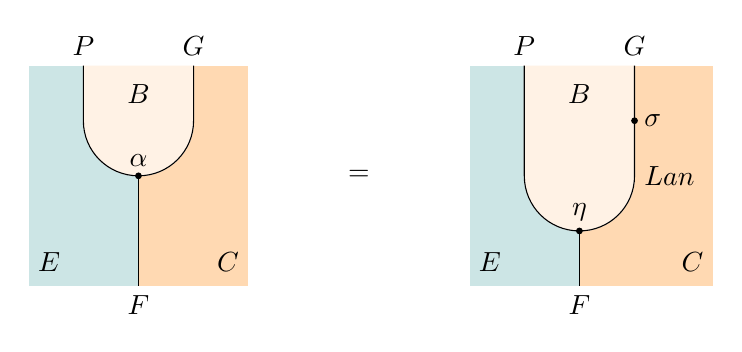
\begin{tikzpicture}
\def \dx {0.7}
\def \dy {-0.7}

\def \xa{-3 * \dx};
\def \xb{-2 * \dx};
\def \xc{-1 * \dx};
\def \xd{0};
\def \xe{1 * \dx};

\def \ya{0};
\def \yb{1 * \dy};
\def \yc{2 * \dy};
\def \yd{3 * \dy};
\def \ye{4 * \dy};

% left background
\filldraw[fill=blue!50!green!20, draw=white] (\xa, \ye) rectangle (\xc, \ya);
% right background
\filldraw[fill=orange!30, draw=white] (\xc, \ye) rectangle (\xe, \ya);
% fill shape\yb
\path [fill=orange!10, draw=white]  (\xb, \ya) to (\xb, \yb) to [out=270, in=180]  (\xc, \yc) to  [out=0, in=270] (\xd, \yb) to (\xd, \ya);

% cup
\draw (\xb, \ya) to (\xb, \yb) to [out=270, in=180]  (\xc, \yc) to  [out=0, in=270] (\xd, \yb) to (\xd, \ya);
\draw (\xc, \yc) -- (\xc, \ye);

% natural transformations
\filldraw[black] (\xc, \yc) circle (1 pt);
\node [above] at (\xc, \yc) {$\alpha$};

% categories
\node[right] at (\xa, \ye + 0.3) {$\cat E$};
\node[left] at (\xe, \ye + 0.3) {$\cat C$};
\node[above] at (\xc, \ya - 0.6) {$\cat B$};
% functors
\node [above] at (\xb, \ya) {$P$};
\node [above] at (\xd, \ya) {$G$};
\node [below] at (\xc, \ye) {$F$};

%-----------------
\node (eq) at (3 * \dx, \yc) {$=$};
% right diagram

\def \xa{5 * \dx};
\def \xb{6 * \dx};
\def \xc{7 * \dx};
\def \xd{8 * \dx};
\def \xe{9 * \dx + 0.3};

% left background
\filldraw[fill=blue!50!green!20, draw=white] (\xa, \ye) rectangle (\xc, \ya);
% right background
\filldraw[fill=orange!30, draw=white] (\xc, \ye) rectangle (\xe, \ya);
% fill shape
\path [fill=orange!10, draw=white]  (\xb, \ya) to (\xb, \yc) to [out=270, in=180]  (\xc, \yd) to  [out=0, in=270] (\xd, \yc) to (\xd, \ya);

% cup
\draw (\xb, \ya) to (\xb, \yc) to [out=270, in=180]  (\xc, \yd) to  [out=0, in=270] (\xd, \yc) to (\xd, \ya);
\draw (\xc, \yd) -- (\xc, \ye);

% natural transformations
\filldraw[black] (\xc, \yd) circle (1 pt);
\node [above] at (\xc, \yd) {$\eta$};

\filldraw[black] (\xd, \yb) circle (1 pt);
\node [right] at (\xd, \yb) {$\sigma$};

% categories
\node[right] at (\xa, \ye + 0.3) {$\cat E$};
\node[left] at (\xe, \ye + 0.3) {$\cat C$};
\node[above] at (\xc, \ya - 0.6) {$\cat B$};
% functors
\node [above] at (\xb, \ya) {$P$};
\node [above] at (\xd, \ya) {$G$};
\node [below] at (\xc, \ye) {$F$};
\node [right] at (\xd, \yc) {$\text{Lan}$};

\end{tikzpicture}
\]

This establishes the one-to-one mapping between two sets of natural transformations. For every $\alpha$ on the left there is a unique $\sigma$ on the right:
\[  [\cat E, \cat C] (F, G \circ P) \cong [\cat B, \cat C](\text{Lan}_P F , G)  \]


\subsection{Left Kan extension as a coend}

Recall the ninja co-Yoneda lemma. For every co-presheaf $F$, we have:
\[ F b \cong \int^{c} \cat B(c, b) \times F c \]
The left Kan extension generalizes this formula to:
\[ (\text{Lan}_P F)\, b \cong \int^{e} \cat B (P e, b) \times F e \]
For a general functor $F \colon \cat E \to \cat C$, we replace the product with the \index{copower}copower:
\[ (\text{Lan}_P F)\, b \cong \int^{e} \cat B(P e, b) \cdot F e \]

As long as the coend in question exists, we can prove this formula by considering a mapping out to some functor $G$. We represent the set of natural transformations as the end over $b$:
\[\int_b \cat C \big(\int^e \cat B(P e, b) \cdot F e, G b\big) \]
Using cocontinuity, we pull out the coend, turning it into an end:
\[\int_b \int_e \cat C \big(\cat B(P e, b) \cdot F e, G b\big) \]
and we plug in the definition of co-power:
\[\int_b \int_e \cat C \big(\cat B(P e, b), \cat C (F e, G b)\big) \]
We can now use the Yoneda lemma to integrate over $b$, replacing $b$ with $P e$:
\[\int_e \cat C (F e, G (P e))\big) \cong  [\cat E, \cat C] (F, G \circ P) \]
This indeed gives us the left adjoint to functor pre-composition:
\[ [\cat B, \cat C](\text{Lan}_P F , G) \cong  [\cat E, \cat C] (F, G \circ P) \]

In $\Set$, the co-power decays to a cartesian product, so we get a simpler formula:
\[ (\text{Lan}_P F)\, b \cong \int^{e} \cat B (P e, b) \times F e \]

 Notice that, if the functor $P$ has a right adjoint, let's call it $P^{-1}$:
 \[ \cat B(P e , b) \cong \cat E(e, P^{-1} b) \]
 we can use the ninja co-Yoneda lemma to get:
 \[  (\text{Lan}_P F)\, b \cong (F \circ P^{-1}) b \]
 thus reinforcing the intuition that a Kan extension inverts $P$ and follows it with $F$.
 
\subsection{Left Kan extension in Haskell}

When translating the formula for the left Kan extension to Haskell, we replace the coend with the existential type. Symbolically:
 \begin{haskell}
type Lan p f b = exists e. (p e -> b, f e)
 \end{haskell}
This is how we would encode the existential using \hask{GADT}'s:
 \begin{haskell}
data Lan p f b where
    Lan :: (p e -> b) -> f e -> Lan p f b
 \end{haskell}
 
 The unit of the left Kan extension is a natural transformation from the functor \hask{f} to the composition of \hask{(Lan p f)} after \hask{p}:
 \begin{haskell}
unit :: forall p f e'. 
    f e' -> Lan p f (p e')
\end{haskell}
To implement the unit, we start with a value of the type \hask{(f e')}. We have to come up with some type \hask{e}, a function \hask{p e -> p e'}, and a value of the type \hask{(f e)}. The obvious choice is to pick \hask{e = e'} and use the identity at \hask{(p e')}:
\begin{haskell}
unit fe = Lan id fe 
\end{haskell}

The computational power of the left Kan extension lies in its universal property. Given a functor \hask{g} and a natural transformation from \hask{f} to the composition of \hask{g} after \hask{p}:
\begin{haskell}
type Alpha p f g = forall e. f e -> g (p e)
\end{haskell}
there is a unique natural transformation $\sigma$ from the corresponding left Kan extension to \hask{g}:
\begin{haskell}
sigma :: Functor g => Alpha p f g -> forall b. (Lan p f b -> g b)
sigma alpha (Lan pe_b fe) = fmap pe_b (alpha fe)
\end{haskell}
that factorizes $\alpha$ through the unit $\eta$:
\[ \alpha = (\sigma \circ P) \cdot \eta \]
The whiskering of $\sigma$ means instantiating it at \hask{b = p e}, so the factorization of $\alpha$ is implemented as:
\begin{haskell}
factorize :: Functor g => Alpha p f g -> f e -> g (p e)
factorize alpha = sigma alpha . unit
\end{haskell}
 \begin{exercise}
Implement the \hask{Functor} instance for \hask{Lan}.
\end{exercise}

\subsection{Colimits as Kan extensions}

Just like limits can be defined as right Kan extensions, colimits can be defined as left Kan extension. 

We start with an indexing category $\cat J$ that defines the shape of the colimit. The functor $D$ selects this shape in the target category $\cat C$. The apex of the cocone is selected by a functor from the terminal single-object category $\Cat 1$. The natural transformation defines a cocone from $D$ to $X$:
\[
 \begin{tikzcd} [row sep=1cm, column sep=1cm]
 \cat J
 \arrow[rr, "D", "" {name=ID, below} ]
 \arrow[d, bend right, "!"']
 && \cat C
 \\
 \Cat 1
  \arrow[urr, bend right, "X"']
 \arrow[Rightarrow, "\gamma",  from=ID]
 \end{tikzcd}
\]

Here's an illustrative example of a simple shape consisting of three objects and three morphisms (not counting identities). The object $x$ is the image of the single object $*$ under the functor $X$:
\[
 \begin{tikzcd}
1 
\arrow[rr, red]
\arrow[rd, red]
&& 2
\arrow[dl, red]
\\
& 3
\\
\\
& *
 \end{tikzcd}
 \qquad
 \begin{tikzcd}
D 1 
\arrow[rr, red]
\arrow[rd, red]
\arrow[dddr, "\gamma_1"']
&& D 2
\arrow[dl, red]
\arrow[dddl, "\gamma_2"]
\\
& D 3
\arrow[dd, "\gamma_3"]
\\
\\
&x
 \end{tikzcd}
 \]
The colimit is the universal cocone, which is given by the left Kan extension of $D$ along the functor $!$:
\[ \text{Colim}\; D = \text{Lan}_! D \]


\subsection{Right adjoint as a left Kan extension}

We've seen that, when we have an adjunction $L \vdash R$, the left adjoint is related to the right Kan extension. Dually, if the right adjoint exists, it can be expressed as the left Kan extension of the identity functor:
\[ R \cong \text{Lan}_L \text{Id} \]
Conversely, if the left Kan extension of identity exists and it preserves the functor $L$:
\[ L \circ \text{Lan}_L \text{Id} \cong \text{Lan}_L L \]
than $\text{Lan}_L \text{Id}$ is the right adjoint of $L$. The left Kan extension of $L$ along itself is called the \index{density comonad} density comonad.



The unit of Kan extension is the same as the unit of the adjunction:
\[
 \begin{tikzcd} [row sep=1cm, column sep=1cm]
 \cat C
 \arrow[rr, "\text{Id}", "" {name=ID, below} ]
 \arrow[d, bend right, "L"']
 && \cat C
 \\
 \cat D
  \arrow[urr, bend right, "R"']
 \arrow[Rightarrow, "\eta",  from=ID]
 \end{tikzcd}
\]
The proof of universality is analogous to the one for the right Kan extension.

\begin{exercise}
Implement the \hask{Comonad} instance for the density comonad:
\begin{haskell}
data Density f c where
   D :: (f d -> c) -> f d -> Density f c
\end{haskell}
\end{exercise}

\subsection{Day convolution as a Kan extension}

We've seen Day convolution defined as a tensor product in the category of co-presheaves over a monoidal category $\cat C$:
\[ (F \star G) c = \int^{a, b} \cat C (a \otimes b, c) \times F a \times G b \]
Co-presheaves, that is functors in $[\cat C, \Set]$, can also be tensored using an \index{external tensor product}\emph{external tensor product}. An external product of two objects, instead of producing an object in the same category, picks an object in a different category. In our case, the product of two functors ends up in the category of co-presheaves on $\cat C \times \cat C$:
\[ \bar{\otimes} \colon [\cat C, \Set] \times [\cat C, \Set] \to [\cat C \times \cat C, \Set] \]
The product of two co-presheaves acting on a pair of objects in $\cat C \times \cat C$, is given by the formula:
\[ (F \bar{\otimes} G)\langle a, b \rangle = F a \times G b \]

It turns out that Day convolution of two functors can be expressed as a left Kan extension of their external product along the tensor product in $\cat C$:
\[ F \star G \cong \text{Lan}_{\otimes} (F \bar{ \otimes } G) \]
Pictorially:
\[
 \begin{tikzcd} [row sep=1cm, column sep=1cm]
 \cat C \times \cat C
 \arrow[rr, "F \bar{\otimes} G", "" {name=ID, below} ]
 \arrow[d, bend right, "\otimes"']
 && \Set
 \\
 \cat C
  \arrow[urr, bend right, "\text{Lan}_{\otimes} (F \bar{ \otimes } G)"']
 \end{tikzcd}
\]

Indeed, using the coend formula for the left Kan extension we get:
\[ (\text{Lan}_{\otimes} (F \bar{ \otimes } G)) c \cong \int^{\langle a, b\rangle} \cat C ( a \otimes b, c) \cdot (F \bar{ \otimes } G)\langle a, b\rangle\]

\[ \cong \int^{\langle a, b\rangle} \cat C ( a \otimes b, c) \cdot (F a \times G  b) \]
Since the two functors are $\Set$-valued, the co-power decays into the cartesian product:
\[ \cong \int^{\langle a, b\rangle} \cat C ( a \otimes b, c) \times F a \times G  b \]
and reproduces the formula for Day convolution.

\section{Useful Formulas}
\begin{itemize}
\item Co-power:
\[ \cat C (A \cdot b, c) \cong \Set \big( A, \cat C (b, c)\big) \]
\item Power:
\[ \cat C (b, A \pitchfork c) \cong \Set  \big(A, \cat C(b, c)\big) \]
\item Right Kan extension:
\[ [\cat E, \cat C](G \circ P, F) \cong [\cat B, \cat C](G, \text{Ran}_P F) \]
 \[ (\text{Ran}_P F) b \cong \int_e \cat B (b, P e) \pitchfork F e \]
\item Left Kan extension:
\[ [\cat B, \cat C](\text{Lan}_P F , G) \cong  [\cat E, \cat C] (F, G \circ P) \]
\[ (\text{Lan}_P F)\, b \cong \int^{e} \cat B(P e, b) \cdot F e \]
\item Right Kan extension in $\Set$:
  \[ (\text{Ran}_P F) b \cong \int_e \Set \big( \cat B (b, P e), F e\big) \]
\item Left Kan extension in $\Set$:
\[ (\text{Lan}_P F) b \cong \int^{e} \cat B (P e, b) \times F e \]


\end{itemize}

\end{document}